\chapter{Description of Data Objects}

\begin{tabular}{llll}
entity  & block         & set        & map    \\
node    &               & nodeset    & nodemap \\
edge    & edgeblock     & edgeset    & edgemap  \\
face    & faceblock     & faceset    & facemap   \\
element & element block & elementset & elementmap \\
\end{tabular}

The data in \exo{} files can be divided into three primary categories:
initialization data, model data, and results data.

Initialization data includes sizing parameters (number of
nodes, number of elements, etc.), optional quality assurance
information (names of codes that have operated on the data),
and optional informational text.

The model is described by data which are static (do not change
through time). This data includes nodal coordinates, element
connectivity (node lists for each element), element attributes,
and node sets and side sets (used to aid in applying loading
conditions and boundary constraints).

The results are optional and include five types of variables -- nodal,
element, nodeset, sideset, and global -- each of which is stored
through time. Nodal results are output (at each time step) for all the
nodes in the model. An example of a nodal variable is displacement in
the X direction. Element, nodeset, and sideset results are output (at
each time step) for all entities (elements, nodes, sides) in one or
more entity block. For example, stress may be an element
variable. Another use of element variables is to record element status
(a binary flag indicating whether each element is "alive" or "dead")
through time. Global results are output (at each time step) for a
single element or node, or for a single property. Linear momentum of a
structure and the acceleration at a particular point are both examples
of global variables. Although these examples correspond to typical FE
applications, the data format is flexible enough to accommodate a
spectrum of uses.

A few conventions and limitations must be cited:
\begin{itemize}
 \item {There are no restrictions on the frequency of results output
 except that the time value associated with each successive time step
 must increase monotonically.}

 \item {To output results at different frequencies (i.e., variable A
 at every simulation time step, variable B at every other time step)
 multiple \exo{} files must be used.}

 \item {There are no limits to the number of each type of results, but
 once declared, the number cannot change. }

 \item {If the mesh geometry changes in time (i.e., number of nodes
 increases, connectivity changes), the new geometry must be output to
 a new \exo{} file.}
\end{itemize}

The following sections describe the data objects that can be stored in
an \exo{} file. API functions that read / write the particular objects
are included for reference. API routines for the C binding are in
lower case. Refer to Section 4 on page 21 for a detailed description
of each API function.

\section{Global Parameters}
\api\cfuncref{ex_put_init}, \cfuncref{ex_get_init}

Every \exo{} file is initialized with the following parameters:

\begin{itemize}
 \item {Title -- data file title of length}
 \param{MAX_LINE_LENGTH}. Refer to discussion below for definition
 of \param{MAX_LINE_LENGTH}.

 \item {Number of nodes -- the total number of nodes in the model.}

 \item {Problem dimensionality -- the number of spatial coordinates
 per node (1, 2, or 3).}

 \item {Number of elements -- the total number of elements of all
 types in the file.}

 \item {Number of element blocks -- within the \exo{} data model,
 elements are grouped together into blocks. Refer to Section 3.8 on
 page 8 for a description of element blocks. }

 \item {Number of node sets -- node sets are a convenient method for
 referring to groups of nodes. Refer to Section 3.9 on page 11 for a
 description of node sets.}

 \item {Number of side sets -- side sets are used to identify elements
 (and their sides) for specific purposes. Refer to Section 3.11 on
 page 12 for a description of side sets.}

 \item Database version number -- the version of the data objects
 stored in the file. This document describes database version is
 \version{}.

 \item API version number -- the version of the \exo{} library
 functions which stored the data in the file. The API version can
 change without changing the database version and vice versa. This
 document describes API version \version{}.

 \item {I/O word size -- indicates the precision of the floating point
 data stored in the file. Currently, four- or eight-byte floating
 point numbers are supported. It is not necessary that an application
 code be written to handle the same precision as the data stored in
 the file. If required, the routines in the \exo{} library perform
 automatic conversion between four- and eight-byte numbers.}

 \item Length of character strings -- all character data stored in an
 \exo{} file is either of length \param{MAX_STR_LENGTH} or
 \param{MAX_LINE_LENGTH}. These two constants are defined in the
 file \file{exodusII.h}. Current values are 32 and
 80, respectively.

 \item Length of character lines -- see description above
for length of character strings.
\end{itemize}


\section{Quality Assurance Data}

\begin{spacing}{1.5}
\api \cfuncref{ex_put_qa}, \cfuncref{ex_get_qa}
\end{spacing}

Quality assurance (QA) data is optional information that can be
included to indicate which application codes have operated on the data
in the file. Any number of QA records can be included, with each
record containing four character strings of length
\param{MAX_STR_LENGTH}. The four character strings are the following
(in order):

\begin{description}

\item[Code name] indicates the application code that has operated
on the \exo{} file.

\item[Code QA descriptor] provides a location for a version
identifier of the application code.

\item[Date] the date on which the application code was executed;
should be in the format 20080331.

 \item[Time] the 24-hour time at which the application code
was executed; should be in the format hours:minutes:seconds,
such as 16:30:15.
 \end{description}


\section{Information Data}


\begin{spacing}{1.5}
\api \cfuncref{ex_put_info}, \cfuncref{ex_get_info}
\end{spacing}

This is for storage of optional supplementary text. Each text record
is of length \param{MAX_LINE_LENGTH}; there is no limit to the
number of text records.


\section{Nodal Coordinates}


\begin{spacing}{1.5}
\api \cfuncref{ex_put_coord}, \cfuncref{ex_get_coord}
\end{spacing}

The nodal coordinates are the floating point spatial coordinates of
all the nodes in the model. The number of nodes and the problem
dimension define the length of this array. The node index cycles
faster than the dimension index, thus the X coordinates for all the
nodes is written before any Y coordinate data are written. Internal
node numbers (beginning with 1) are implied from a nodes's place in
the nodal coordinates record. See Section~\ref{s:nnm} for a discussion
of internal node numbers.

\subsection{Coordinate Names}

\begin{spacing}{1.5}
\api \cfuncref{ex_put_coord_names}, \cfuncref{ex_get_coord_names}
\end{spacing}

The coordinate names are character strings of length
\param{MAX_STR_LENGTH} which name the spatial coordinates. There is
one string for each dimension in the model, thus there are one to
three strings.


\section{Node Number Map}\label{s:nnm}

\begin{spacing}{1.5}
\api \cfuncref{ex_put_node_num_map}, \cfuncref{ex_get_node_num_map}


\end{spacing}

Within the data model, internal node IDs are indices into
the nodal coordinate array and internal element IDs are indices
into the element connectivity array. Thus, internal node and
element numbers (IDs) are contiguous (i.e., 1\ldots{number_of_nodes}
and 1\ldots{number_of_elements}, respectively). Optional
node and element number maps can be stored to relate user-defined
node and element IDs to these internal node and element numbers.
The length of these maps are {number_of_nodes} and {number_of_elements},
respectively. As an example, suppose a database contains exactly
one QUAD element with four nodes. The user desires the element
ID to be 100 and the node IDs to be 10, 20, 30, and 40 as shown
in  Figure~\ref{f:UserDefinedNodeElementIds}.
\begin{figure}[htbp]
\begin{center}
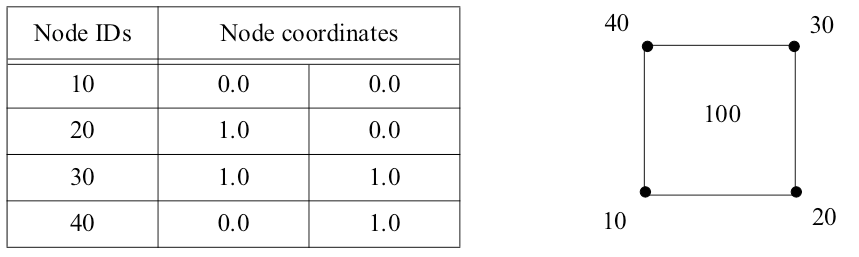
\includegraphics[width=5.972in, height=2.486in]{figures/UserDefinedNodeElementIds.png}
\caption{User-defined Node and Element IDs.}\label{f:UserDefinedNodeElementIds}
\end{center}
\end{figure}

The internal data structures representing the above model
would be the following:


\begin{itemize}
 \item {nodal coordinate array}{:} {(0.0, 1.0, 1.0,
0.0, 0.0, 0.0, 1.0, 1.0)}

 \item {connectivity array}{: (1, 2, 3, 4)}

 \item {node number map}{: (10, 20, 30, 40)}

 \item {element number map}{: (100)}
\end{itemize}


Internal (contiguously numbered) node and element IDs must be used for
all data structures that contain node or element numbers (IDs),
including node set node lists, side set element lists, and element
connectivity. Additionally, to inquire the value(s) of node or element
results variables, an application code must pass the internal node or
element number for the node or element of interest.




\section{Element Number Map}\label{s:enm}

\begin{spacing}{1.5}
\api \cfuncref{ex_put_elem_num_map}, \cfuncref{ex_get_elem_num_map}


\end{spacing}

{Refer to  Section 3.5 for a discussion of the optional element
number map.}




\section{Optimized Element Order Map}\label{s:eom}

\begin{spacing}{1.5}
\api \cfuncref{ex_put_map}, \cfuncref{ex_get_map}


\end{spacing}

The optional element order map defines the element order in which a
solver (e.g., a wavefront solver) should process the elements. For
example, the first entry is the number of the element which should be
processed first by the solver. The length of this map is the total
number of elements in the model.

\section{Element Blocks}

For efficient storage and to minimize I/O, elements are grouped into
element blocks. Within an element block, all elements are of the same
type (basic geometry and number of nodes). This definition does not
preclude multiple element blocks containing the same element type
(i.e., ``QUAD'' elements may be in more than one element block); only
that each element block may contain only one element type.

The internal number of an element numbering is defined implicitly by
the order in which it appears in the file. Elements are numbered
internally (beginning with 1) consecutively across all element
blocks. See Section~\ref{s:enm} for a discussion of internal element
numbering.

\subsection{Element Block Parameters}\label{s:ebp}

\begin{spacing}{1.5}
\api \cfuncref{ex_put_elem_block}, \cfuncref{ex_get_elem_block}, \cfuncref{ex_get_elem_blk_ids}
\end{spacing}

The following parameters are defined for each element block:

\begin{itemize}
 \item element block ID -- an arbitrary, unique, positive integer
 which identifies the particular element block. This ID is used as a
 ``handle'' into the database that allows users to specify a group of
 elements to the application code without having to know the order in
 which element blocks are stored in the file.

 \item element type Element type -- a character string of length
 \param{MAX_STR_LENGTH} to distinguish element types. All elements
 within the element block are of this type. Refer to
 Table~\ref{t:element_types} on page~\pageref{t:element_types} for a
 list of names that are currently accepted. It should be noted that
 the \exo{} library routines do not verify element type names against
 a standard list; the interpretation of the element type is left to
 the application codes which read or write the data. In general, the
 first three characters uniquely identify the element
 type. Application codes can append characters to the element type
 string (up to the maximum length allowed) to further classify the
 element for specific purposes.

 \item {Number of elements -- the number of elements in the
element block.}

 \item {Nodes per element -- the number of nodes per element
for the element block.}

 \item {Number of attributes -- the number of attributes per element
 in the element block. See below for a discussion of element
 attributes.}
\end{itemize}



\subsection{Element Connectivity}

\begin{spacing}{1.5}
\api \cfuncref{ex_put_elem_conn}, \cfuncref{ex_get_elem_conn}
\end{spacing}

The element connectivity contains the list of nodes (internal node
IDs; see Section~\ref{s:enm} for a discussion of node IDs) which
define each element in the element block. The length of this list is
the product of the number of elements and the number of nodes per
element as specified in the element block parameters. The node index
cycles faster than the element index. Node ordering follows the
conventions illustrated in Figures~\ref{topology:1d}
through~\ref{topology:hex27}. The node ordering conventions follow the element topology
used in \code{PATRAN}~\cite{PATRAN}. Thus, for higher-order elements
than those illustrated, use the ordering prescribed in the
\code{PATRAN} User
Manual~\url{http://web.mscsoftware.com/training_videos/patran/reverb3/index.html#page/Finite%2520Element%2520Modeling/elem_lib_topics.16.1.html#ww33606}. For
elements of type CIRCLE or SPHERE, the topology is one node at the
center of the circle or sphere element.

\begin{figure}
\centering
\subcaptionbox{Circle\label{topology:circle}}
{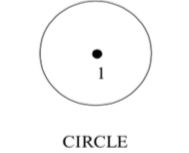
\includegraphics{topology/circle.png}}
\subcaptionbox{Sphere\label{topology:sphere}}
{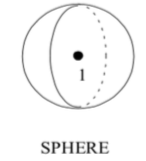
\includegraphics{topology/sphere.png}}
\caption{Node Ordering for Circle and Sphere Elements}\label{topology:1d}
\end{figure}


\begin{figure}
\begin{center}
\subcaptionbox{Bar2\label{topology:bar2}}
{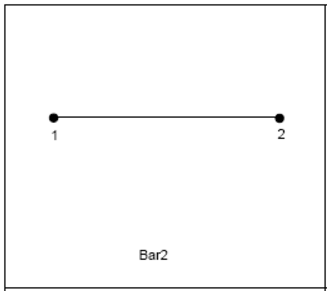
\includegraphics[width=2.000in, height=2.000in]{topology/bar2.png}}
\subcaptionbox{Bar3\label{topology:bar3}}
{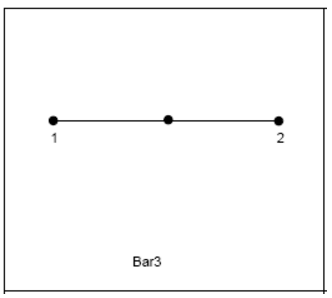
\includegraphics[width=2.000in, height=2.000in]{topology/bar3.png}}
\caption{Node Ordering for Bar/Truss/Beam Elements}
\end{center}
\end{figure}


\begin{figure}
\begin{center}
\subcaptionbox{Tri3\label{topology:tri3}}
{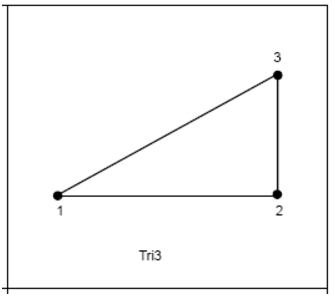
\includegraphics[width=2.000in, height=2.000in]{topology/tri3.png}}
\subcaptionbox{Tri4\label{topology:tri4}}
{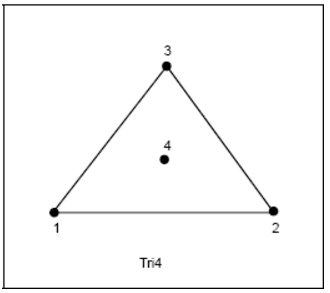
\includegraphics[width=2.000in, height=2.000in]{topology/tri4.png}}
\subcaptionbox{Tri6\label{topology:tri6}}
{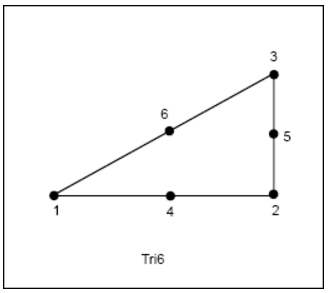
\includegraphics[width=2.000in, height=2.000in]{topology/tri6.png}}
\subcaptionbox{Tri7\label{topology:tri7}}
{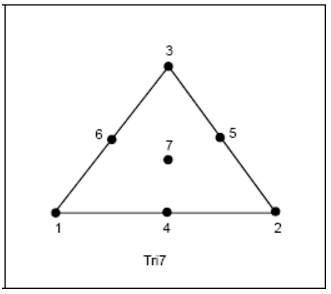
\includegraphics[width=2.000in, height=2.000in]{topology/tri7.png}}
\caption{Node Ordering for Triangular Elements.}
\end{center}
\end{figure}


\begin{figure}
\begin{center}
\subcaptionbox{Quad4\label{topology:quad4}}
{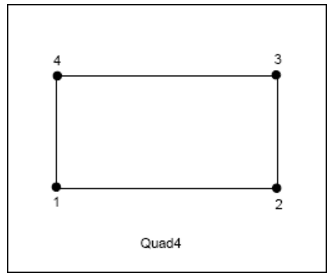
\includegraphics[width=2.9in, height=2.9in]{topology/quad4.png}}
\subcaptionbox{Quad5\label{topology:quad5}}
{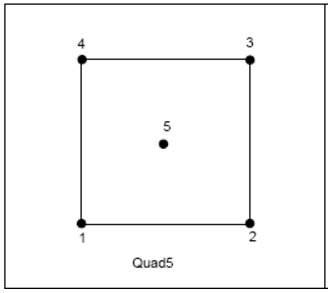
\includegraphics[width=2.9in, height=2.9in]{topology/quad5.png}}
\subcaptionbox{Quad8\label{topology:quad8}}
{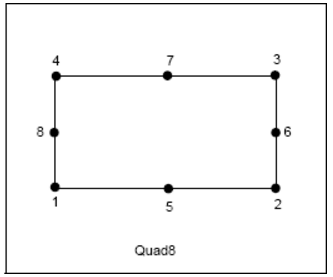
\includegraphics[width=2.9in, height=2.9in]{topology/quad8.png}}
\subcaptionbox{Quad9\label{topology:quad9}}
{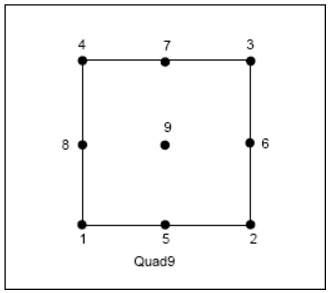
\includegraphics[width=2.9in, height=2.9in]{topology/quad9.png}}
\caption{Node Ordering for Quadrilateral Elements.}\label{topology:quad}
\end{center}
\end{figure}

\begin{figure}
\begin{center}
\subcaptionbox{Tet4\label{topology:tet04}}
{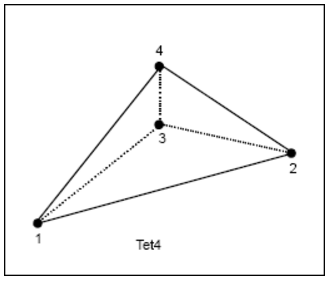
\includegraphics[width=2.9in, height=2.9in]{topology/tet04.png}}
\subcaptionbox{Tet5\label{topology:tet05}}
{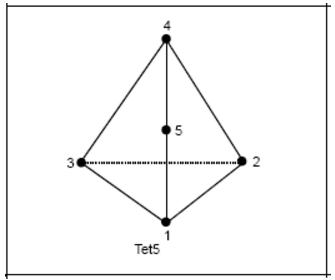
\includegraphics[width=2.9in, height=2.9in]{topology/tet05.png}}
\subcaptionbox{Tet10\label{topology:tet10}}
{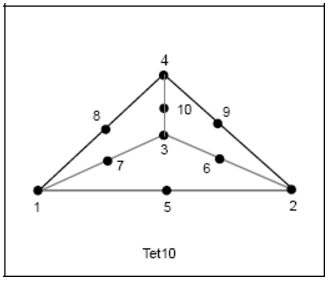
\includegraphics[width=2.9in, height=2.9in]{topology/tet10.png}}
\subcaptionbox{Tet11\label{topology:tet11}}
{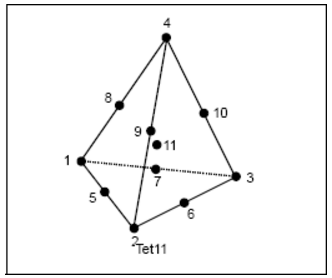
\includegraphics[width=2.9in, height=2.9in]{topology/tet11.png}}
\caption{Node Ordering for Tetrahedral Elements.}\label{topology:tet}
\end{center}
\end{figure}

\begin{figure}
\begin{center}
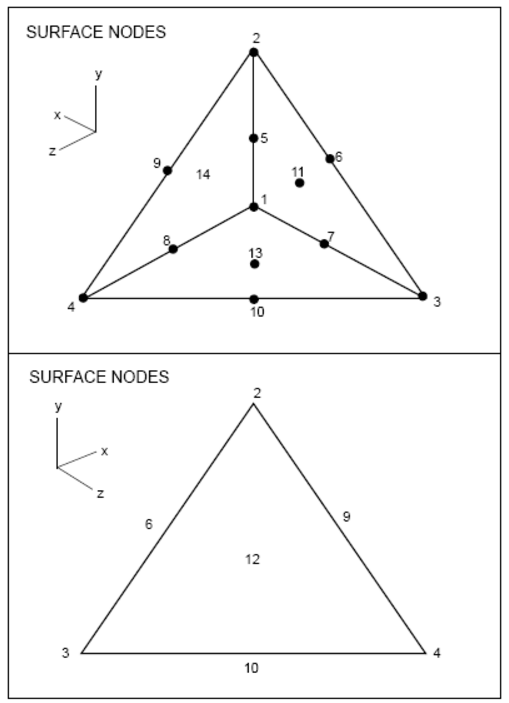
\includegraphics[width=5.000in, height=5.000in]{topology/tet14.png}
\caption{Node Ordering for Tetrahedral Tet14 Element.}\label{topology:tet14}
\end{center}
\end{figure}


\begin{figure}
\begin{center}
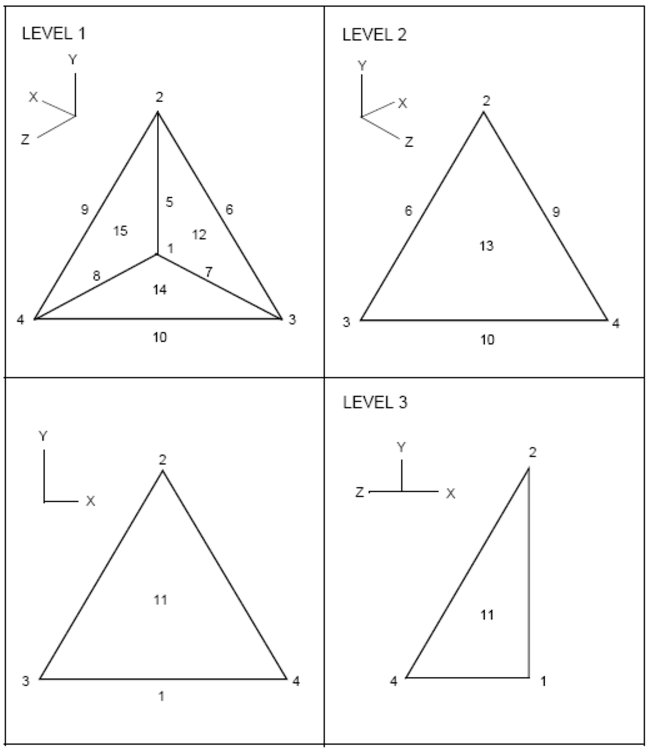
\includegraphics[width=5.000in, height=5.000in]{topology/tet15.png}
\caption{Node Ordering for Tetrahedral Tet15 Element.}\label{topology:tet15}
\end{center}
\end{figure}

\begin{figure}
\begin{center}
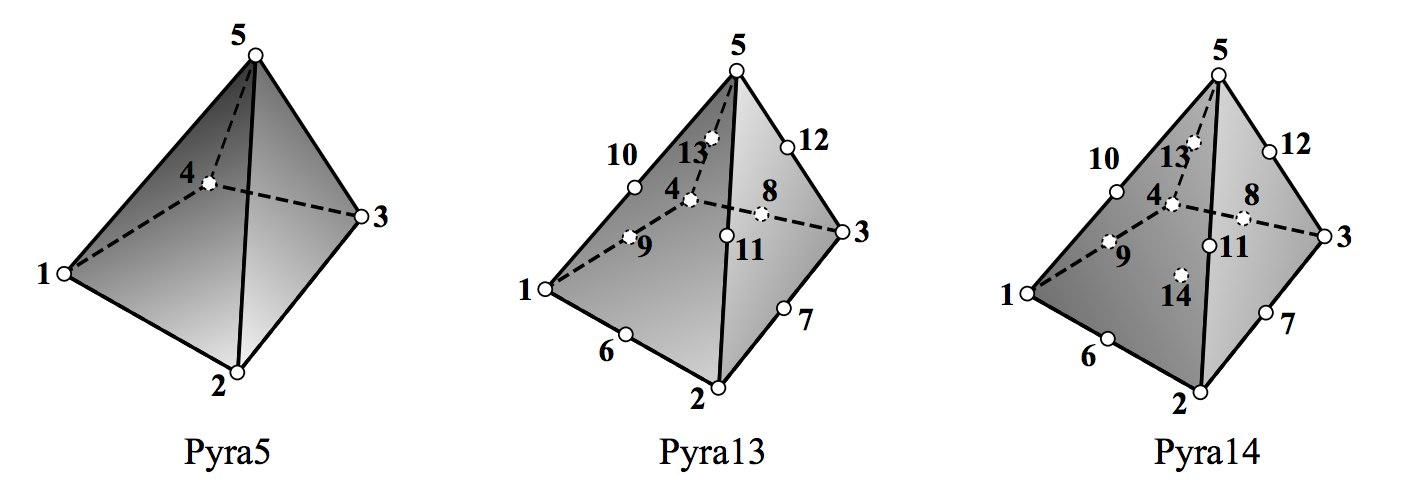
\includegraphics[width=6.000in, height=2.1in]{topology/pyramid.png}
\caption{Node Ordering for Pyramid Elements (pyramid5, pyramid13, pyramid14).}\label{topology:pyramid}
\end{center}
\end{figure}


\begin{figure}
\begin{center}
\subcaptionbox{Wedge6\label{topology:wedge06}}
{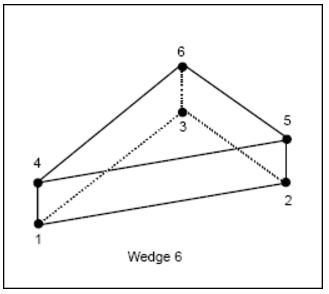
\includegraphics[width=1.9in, height=1.9in]{topology/wedge06.png}}
\subcaptionbox{Wedge15\label{topology:wedge15}}
{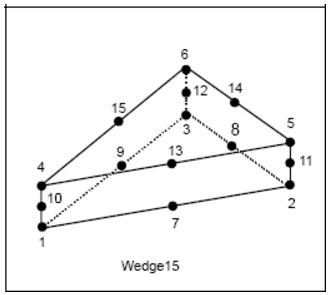
\includegraphics[width=1.9in, height=1.9in]{topology/wedge15.png}}
\subcaptionbox{Wedge16\label{topology:wedge16}}
{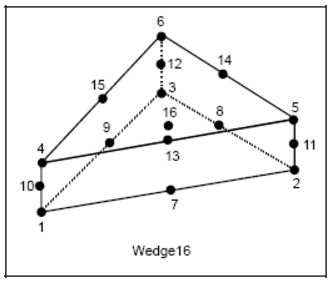
\includegraphics[width=1.9in, height=1.9in]{topology/wedge16.png}}
\caption{Node Ordering for Wedge Elements.}\label{topology:wedge}
\end{center}
\end{figure}

\begin{figure}
\begin{center}
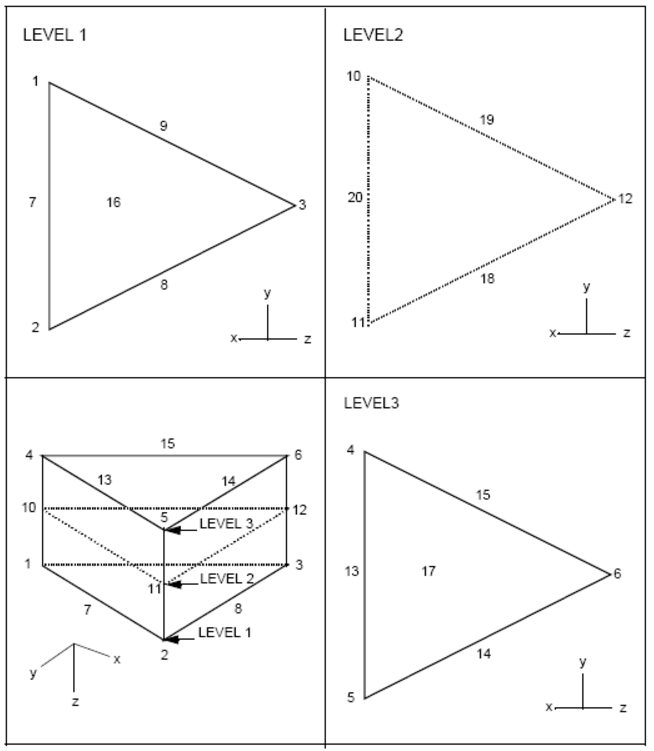
\includegraphics[width=6.000in, height=6.000in]{topology/wedge20.png}
\caption{Node Ordering for Wedge Elements (Wedge20).}\label{topology:wedge20}
\end{center}
\end{figure}


\begin{figure}
\begin{center}
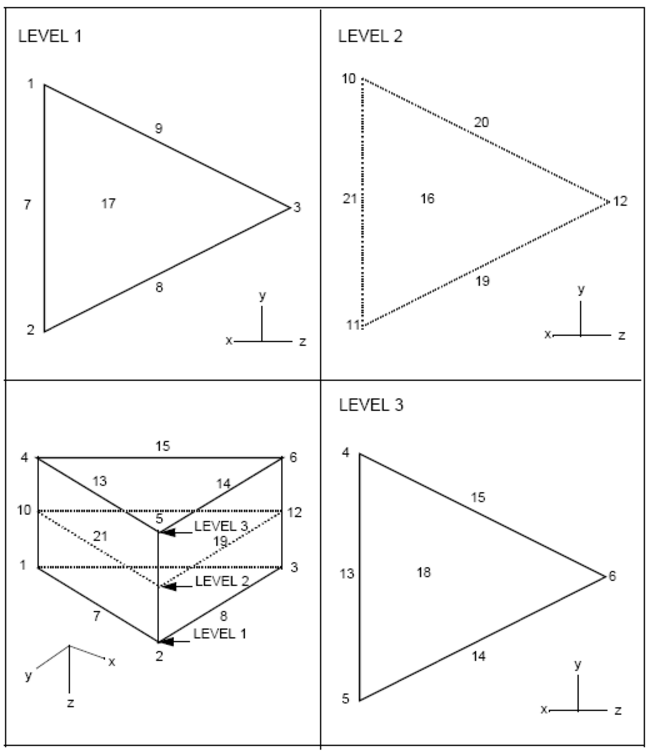
\includegraphics[width=6.000in, height=6.000in]{topology/wedge21.png}
\caption{Node Ordering for Wedge Elements (Wedge21).}\label{topology:wedge21}
\end{center}
\end{figure}

\begin{figure}
\begin{center}
\subcaptionbox{Hex8\label{topology:hex8}}
{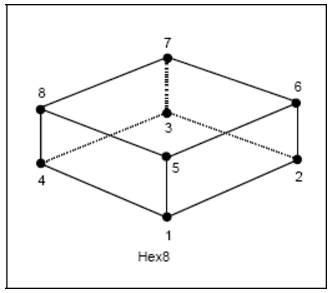
\includegraphics[width=1.9in, height=1.9in]{topology/hex08.png}}
\subcaptionbox{Hex9\label{topology:hex9}}
{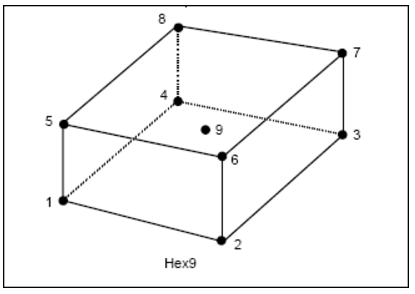
\includegraphics[width=1.9in, height=1.9in]{topology/hex09.png}}
\subcaptionbox{Hex20\label{topology:hex20}}
{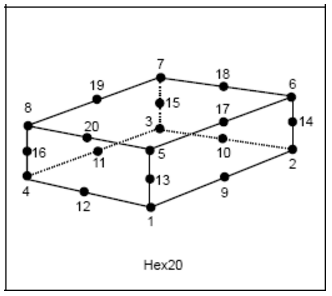
\includegraphics[width=1.9in, height=1.9in]{topology/hex20.png}}
\caption{Node Ordering for Hexahedral Elements.}\label{topology:hex}
\end{center}
\end{figure}

\begin{figure}
\begin{center}
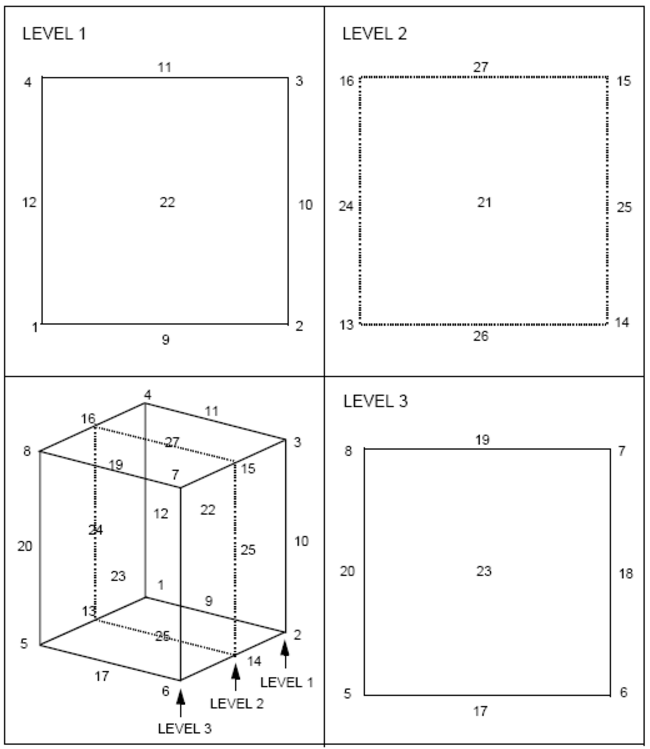
\includegraphics[width=6.000in, height=6.000in]{topology/hex27.png}
\caption{Node Ordering for Hexahedral Elements (Hex27).}\label{topology:hex27}
\end{center}
\end{figure}


\subsection{Element Attributes}

\begin{spacing}{1.5}
\api \cfuncref{ex_put_elem_attr}, \cfuncref{ex_get_elem_attr}
\end{spacing}

{Element attributes are optional floating point numbers that can be
assigned to each element. Every element in an element block must have
the same number of attributes (as specified in the element block
parameters) but the attributes may vary among elements within the
block. The length of the attributes array is thus the product of the
number of attributes per element and the number of elements in the
element block.  Table~\ref{t:element_types} lists the standard
attributes for the given element types. }

\begin{table}[htbp]
\begin{center}
\begin{tabular}{|l|l|} \hline
Element Type & Attributes \\ \hline
CIRCLE   & R \\ \hline
SPHERE   & R \\ \hline
TRUSS    & A \\ \hline
BEAM     & 2D: A, I, J \\
         & 3D: A, $I_1$, $I_2$, J, $V_1$, $V_2$, $V_3$ \\ \hline
TRIANGLE & \\ \hline
QUAD     & \\ \hline
SHELL    & T \\ \hline
TETRA    & \\ \hline
PYRAMID  & \\ \hline
WEDGE    & \\ \hline
HEX      & \\ \hline
\end{tabular}
\caption{Standard Element Types and Attributes}\label{t:element_types}
\end{center}
\end{table}

\section{Node Sets}

Node sets provide a means to reference a group of nodes with a single
ID. Node sets may be used to specify load or boundary
conditionsboundary conditions, or to identify nodes for a special
output request. A particular node may appear in any number of node
sets, but may be in a single node set only once. (This restriction is
not checked by \exo{} routines.) Node sets may be accessed
individually (using node set parameters, node set node list, and node
set distribution factors) or in a concatenated format (described in
Section 3.10 on page 11). The node sets data are stored identically in
the data file regardless of which method (individual or concatenated)
was used to output them.

\subsection{Node Set Parameters}

\begin{spacing}{1.5}
\api \cfuncref{ex_put_node_set_param}, \cfuncref{ex_get_node_set_param}, \cfuncref{ex_get_node_set_ids}
\end{spacing}

{The following parameters define each node set:}

\begin{itemize}
 \item {node set ID -- a unique positive integer that identifies the
 node set.}

 \item {Number of nodes -- the number of nodes in the node
set.}

 \item {Number of node set distribution factors -- this should be zero
 if there are no distribution factors for the node set. If there are
 any distribution factors, this number must equal the number of nodes
 in the node set since the factors are assigned at each node. Refer to
 the discussion of distribution factors below.}
\end{itemize}



\subsection{Node Set Node List}

\begin{spacing}{1.5}
\api \cfuncref{ex_put_node_set}, \cfuncref{ex_get_node_set}
\end{spacing}

{This is an integer list of all the nodes in the node set. Internal
node IDs (see Section~\ref{s:enm}) must be used in this list.}



\subsection{Node Set Distribution Factors}

\begin{spacing}{1.5}
\api \cfuncref{ex_put_node_set_dist_fact}, \cfuncref{ex_get_node_set_dist_fact}
\end{spacing}

{This is an optional list of floating point factors associated with
the nodes in a node set. These data may be used as multipliers on
applied loads. If distribution factors are stored, each entry in this
list is associated with the corresponding entry in the node set node
list.}


\section{Concatenated Node Sets}

\begin{spacing}{1.5}
\api \cfuncref{ex_put_concat_node_sets}, \cfuncref{ex_get_concat_node_sets}
\end{spacing}

Concatenated node sets provide a means of writing/reading all node
sets with one function call. This is more efficient because it avoids
some I/O overhead, particularly when considering the intricacies of
the \code{NetCDF} library. (Refer to Appendix A for a discussion of
efficiency concerns.) This is accomplished with the following lists:

\begin{itemize}

 \item Node sets IDs -- list (of length number of node sets)
of unique integer node set ID's. The \textit{{i}}\th{} entry in
this list specifies the ID of the \textit{{i}}\th{} node set.

 \item Node sets node counts -- list (of length number of
node sets) of counts of nodes for each node set. Thus, the \textit{{i}}\th{}
entry in this list specifies the number of nodes in the \textit{{i}}\th{}
node set.

 \item Node sets distribution factors counts -- list (of
length number of node sets) of counts of distribution factors
for each node set. The \textit{{i}}\th{} entry in this list specifies
the number of distribution factors in the \textit{{i}}\th{} node
set.

 \item Node sets node pointers -- list (of length number
of node sets) of indices which are pointers into the node sets
node list locating the first node of each node set. The \textit{{i}}\th{}
entry in this list is an index in the node sets node list where
the first node of the \textit{{i}}\th{} node set can be located.

 \item Node sets distribution factors pointers -- list (of
length number of node sets) of indices which are pointers into
the node sets distribution factors list locating the first factor
of each node set. The \textit{{i}}\th{} entry in this list is an
index in the node sets distribution factors list where the first
factor of the \textit{{i}}\th{} node set can be located.

 \item Node sets node list -- concatenated integer list of the nodes
 in all the node sets. Internal node IDs (see Section~\ref{s:enm})
 must be used in this list. The node sets node pointers and node sets
 node counts are used to find the first node and the number of nodes
 in a particular node set.

 \item Node sets distribution factors list -- concatenated
list of the (floating point) distribution factors in all the
node sets. The node sets distribution factors pointers and node
sets distribution factors counts are used to find the first factor
and the number of factors in a particular node set.

\end{itemize}

To clarify the use of these lists, refer to the coding examples
in  Section 4.2.25 and  Section 4.2.26.

\section{Side Sets}

Side sets provide a second means of applying load and boundary
conditions to a model. Unlike node sets, side sets are related to
specified sides of elements rather than simply a list of nodes. For
example, a pressure load must be associated with an element edge (in
2-d) or face (in 3-d) in order to apply it properly. Each side in a
side set is defined by an element number and a local edge (for 2-d
elements) or face (for 3-d elements) number. The local number of the
edge or face of interest must conform to the conventions as
illustrated in Figure~\ref{f:SideSetNumbering}.
\begin{figure}[htbp]
\begin{center}
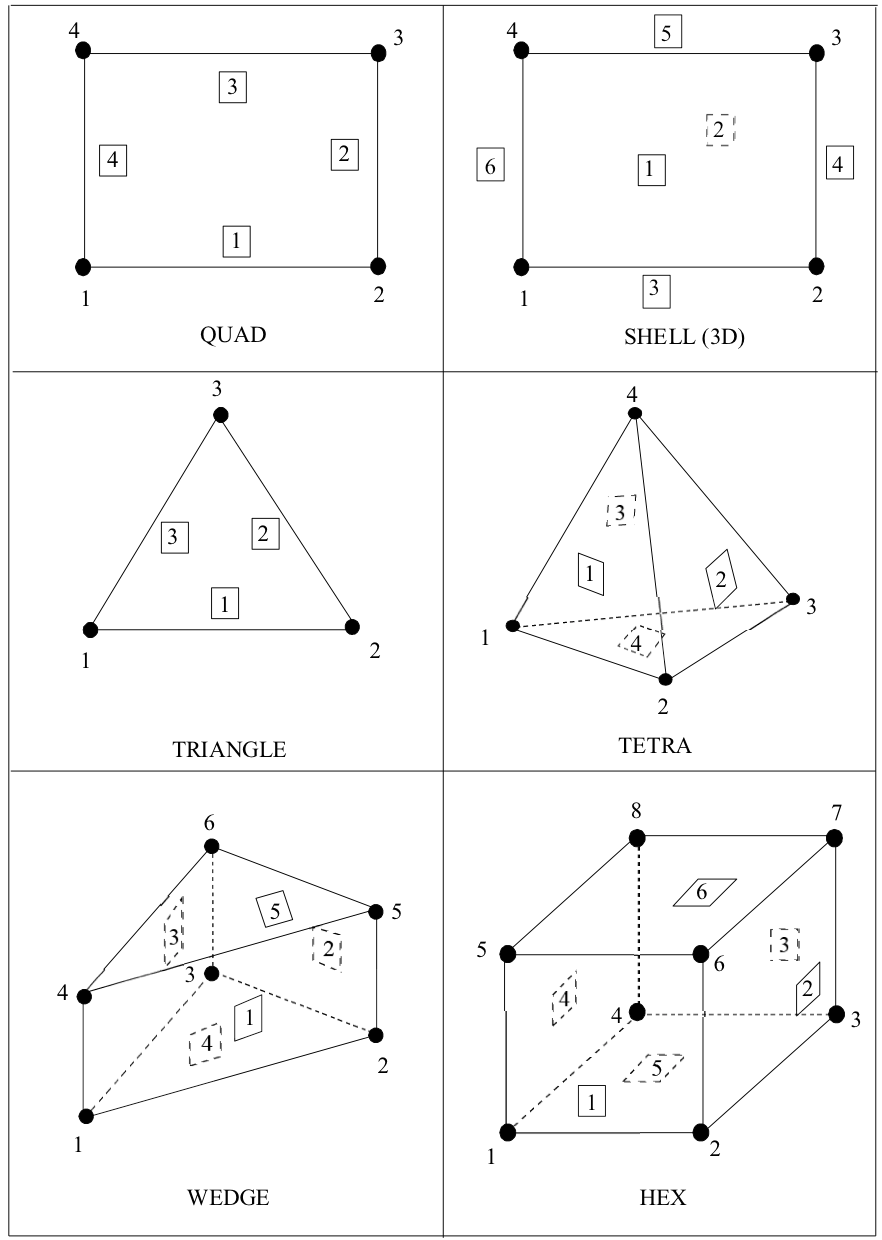
\includegraphics[width=6.250in, height=8.000in]{figures/SideSetNumbering.png}
\caption{Side Set Side Numbering.}\label{f:SideSetNumbering}
\end{center}
\end{figure}

 In this figure, side set side numbers are enclosed in boxes; only the
 essential node numbers to describe the element topology are shown. A
 side set may contain sides of differing types of elements that are
 contained in different element blocks. For instance, a single side
 set may contain faces of WEDGE elements, HEX elements, and TETRA
 elements.



\subsection{Side Set Parameters}



\begin{spacing}{1.5}
\api \cfuncref{ex_put_side_set_param}, \cfuncref{ex_get_side_set_param}, \cfuncref{ex_get_side_set_ids}
\end{spacing}

{The following parameters define each side set:}

\begin{itemize}
 \item {side set ID -- a unique positive integer that identifies the
 side set.}

 \item {Number of sides -- the number of sides in the side
set.}

 \item {Number of side set distribution factors -- this should be zero
 if there are no distribution factors for the side set. If there are
 any distribution factors, they are assigned at the nodes on the sides
 of the side set. Refer to the discussion of distribution factors
 below.}
\end{itemize}

\subsection{Side Set Element List}



\begin{spacing}{1.5}
\api \cfuncref{ex_put_side_set}, \cfuncref{ex_get_side_set}
\end{spacing}

{This is an integer list of all the elements in the side set.
Internal element IDs (see  Section~\ref{s:enm}) must be used
in this list.}



\subsection{Side Set Side List}



\begin{spacing}{1.5}
\api \cfuncref{ex_put_side_set}, \cfuncref{ex_get_side_set}
\end{spacing}

{This is an integer list of all the sides in the side set.
This list contains the local edge (for 2-d elements) or face
(for 3-d elements) numbers following the conventions specified
in  Figure 5.}



\subsection{Side Set Node List}



\begin{spacing}{1.5}
\api \cfuncref{ex_get_side_set_node_list}
\end{spacing}

It is important to note that the nodes on a side set are
not explicitly stored in the data file, but can be extracted
from the element numbers in the side set element list, local
side numbers in the side set side list, and the element connectivity
array. The node IDs that are output are internal node numbers
(see  Section~\ref{s:nnm}). They are extracted according to
the following conventions:


\begin{enumerate}
\item {All nodes for the first side (defined by the first element
in the side set element list and the first side in the side set side
list) are output before the nodes for the second side. There is no
attempt to consolidate nodes; if a node is attached to four different
faces, then the same node number will be output four times -- once
each time the node is encountered when progressing along the side
list.}

\item {The nodes for a single face (or edge) are ordered to assist
an application code in determining an ``outward'' direction. Thus, the
node list for a face of a 3-d element proceeds around the face so that
the outward normal follows the right-hand rule. The node list for an
edge of a 2-d element proceeds such that if the right hand is placed
in the plane of the element palm down, thumb extended with the index
(and other fingers) pointing from one node to the next in the list,
the thumb points to the inside of the element. This node ordering is
detailed in Table~\ref{t:sset_node_ordering} on
page~\pageref{t:sset_node_ordering}}

\item {The nodes required for a first-order element are output
first, followed by the nodes of a higher ordered
element. Table~\ref{t:sset_node_ordering} lists the nodes for
first-order elements.  Refer to the node orderings shown in
Figures~\ref{topology:1d} to ~\ref{topology:hex27} for the additional
nodes on higher-order elements. If a face has a mid-face node, it is
listed last following all mid-edge nodes.  For example, the node
ordering for side~1 of the \code{hex27} element is {1,2,6,5,9,14,17,13,26}}
\end{enumerate}

\begin{table}
\begin{center}
% use packages: array
\begin{tabular}{l|c|lll}
\hline \textbf{Element Type} & \textbf{Side \#}& \textbf{Node Order} \\ \hline
QUAD   & 1 & 1, 2, & 5 \\
(2D)   & 2 & 2, 3, & 6 \\
       & 3 & 3, 4, & 7 \\
       & 4 & 4, 1, & 8 \\ \hline
SHELL  & 1 & 1, 2, 3, 4, & 5, 6, 7, 8, & 9 \\
       & 2 & 1, 4, 3, 2, & 8, 7, 6, 5, & 9 \\
(Edges)& 3 & 1, 2, & 5 \\
       & 4 & 2, 3, & 6 \\
       & 5 & 3, 4, & 7 \\
       & 6 & 4, 1, & 8 \\ \hline
TRIANGLE&1 & 1, 2, & 4 \\
(2D)   & 2 & 2, 3, & 5 \\
       & 3 & 3, 1, & 6 \\ \hline
TRIANGLE& 1 & 1, 2, 3, & 4, 5, 6 \\
(Shell)& 2 & 1, 3, 2, & 6, 5, 4 \\
       & 3 & 1, 2,    & 4  \\
       & 4 & 2, 3,    & 5 \\
       & 5 & 3, 1,    & 6 \\ \hline
TETRA  & 1 & 1, 2, 4, & 5, 9, 8 \\
       & 2 & 2, 3, 4, & 6, 10, 9 \\
       & 3 & 1, 4, 3, & 8, 10, 7 \\
       & 4 & 1, 3, 2, & 7, 6, 5 \\ \hline
WEDGE  & 1 & 1, 2, 5, 4, & 7, 11, 13, 10 \\
       & 2 & 2, 3, 6, 5, & 8, 12, 14, 11 \\
       & 3 & 1, 4, 6, 3, & 10, 15, 12, 9 \\
       & 4 & 1, 3, 2, & 9, 8, 7 \\
       & 5 & 4, 5, 6, & 13, 14, 15 \\ \hline
HEX    & 1 & 1, 2, 6, 5, & 9, 14, 17, 13, & 26 \\
       & 2 & 2, 3, 7, 6, & 10, 15, 18, 14, & 25 \\
       & 3 & 3, 4, 8, 7, & 11, 16, 19, 15, & 27 \\
       & 4 & 1, 5, 8, 4, & 13, 20, 16, 12, & 24 \\
       & 5 & 1, 4, 3, 2, & 12, 11, 10, 9, & 22 \\
       & 6 & 5, 6, 7, 8, & 17, 18, 19, 20, & 23 \\ \hline
PYRAMID&1 & 1, 2, 5, & 6, 11, 10 \\
       & 2 & 2, 3, 5, & 7, 12, 11 \\
       & 3 & 3, 4, 5, & 8, 13, 12 \\
       & 4 & 4, 1, 5, & 9, 10, 13 \\
       & 5 & 1, 4, 3, 2, & 9, 8, 7, 6
\end{tabular}
\caption{Sideset Node Ordering}\label{t:sset_node_ordering}
\end{center}
\end{table}

\subsection{Side Set Node Count List}


\begin{spacing}{1.5}
\api \cfuncref{ex_get_side_set_node_list}
\end{spacing}

The length of the side set node count list is the length of the side
set element list. For each entry in the side set element list, there
is an entry in the side set side list, designating a local side
number. The corresponding entry in the side set node count list is the
number of nodes which define the particular side. In conjunction with
the side set node list, this node count array provides an unambiguous
nodal description of the side set.

\subsection{Side Set Distribution Factors}


\begin{spacing}{1.5}
\api \cfuncref{ex_put_side_set_dist_fact}, \cfuncref{ex_get_side_set_dist_fact}
\end{spacing}

This is an optional list of floating point factors associated with the
nodes on a side set. These data may be used for uneven application of
load or boundary conditions. Because distribution factors are assigned
at the nodes, application codes that utilize these factors must read
the side set node list. The distribution factors must be
stored/accessed in the same order as the nodes in the side set node
list; thus, the ordering conventions described above apply.


\section{Concatenated Side Sets}

\begin{spacing}{1.5}
\api \cfuncref{ex_put_concat_side_sets}, \cfuncref{ex_get_concat_side_sets}
\end{spacing}

Concatenated side sets provide a means of writing / reading all side
sets with one function call. This is more efficient because it avoids
some I/O overhead, particularly when considering the intricacies of
the \code{NetCDF} library. This is accomplished with the following
lists:
\begin{itemize}
 \item {Side sets IDs -- list (of length number of side sets) of
 unique positive integer side set ID's. The} \textit{{i}}{th entry in
 this list specifies the ID of the} \textit{{i}}{th side set.}

 \item {Side sets side counts -- list (of length number of side sets)
 of counts of sides for each side set. Thus, the} \textit{{i}}{th
 entry in this list specifies the number of sides in the}
 \textit{{i}}{th node set. This also defines the number of elements in
 each side set.}

 \item {Side sets distribution factors counts -- list (of length
 number of side sets) of counts of distribution factors for each side
 set. The} \textit{{i}}{th entry in this list specifies the number of
 distribution factors in the} \textit{{i}}{th side set.}

 \item {Side sets side pointers -- list (of length number of side
 sets) of indices which are pointers into the side sets element list
 (and side list) locating the first element (or side) of each side
 set. The} \textit{{i}}{th entry in this list is an index in the side
 sets element list (and side list) where the first element (or side)
 of the} \textit{{i}}{th side set can be located.}

 \item {Side sets distribution factors pointers -- list (of length
 number of side sets) of indices which are pointers into the side sets
 distribution factors list locating the first factor of each side
 set. The} \textit{{i}}{th entry in this list is an index in the side
 sets distribution factors list where the first factor of the}
 \textit{{i}}{th side set can be located.}

 \item {Side sets element list -- concatenated integer list of the
 elements in all the side sets.} {Internal element IDs (see
 Section~\ref{s:enm}) must be used in this list.} {The side sets side
 pointers and side sets side counts are used to find the first element
 and the number of elements in a particular side set.}

 \item {Side sets side list -- concatenated integer list of the sides
 in all the side sets. The side sets side pointers and side sets side
 counts are used to find the first side and the number of sides in a
 particular side set.}

 \item {Side sets distribution factors list -- concatenated list of
 the (floating point) distribution factors in all the side sets. The
 side sets distribution factors pointers and side sets distribution
 factors counts are used to find the first factor and the number of
 factors in a particular side set.}
\end{itemize}



\subsection{Object Properties}

Certain \exo{} objects (currently element blocks, node
sets, and side sets) can be given integer properties, providing
the following capabilitities:
\begin{enumerate}
\item assign a specific integer value to a named property of
an object.

\item tag objects as members of a group. For example element
blocks 1 and 3 and side sets 1 and 2 could be put in a group
named ``TOP.''
\end{enumerate}

This functionality is illustrated in Table~\ref{t:property} which
contains the property values of a sample
\exo{} file with three element blocks, one node set, and two
side sets. Note that an application code can define properties
to be valid for only specified object types. In this example,
``STEEL'' and ``COPPER'' are valid for all element blocks but are
not defined for node sets and side sets.

\begin{table}
\begin{center}
\begin{tabular}{l|cccccc} \hline
Name   & EB 1 & EB 2 & EB 3 & NS 1 & SS 1 & SS 2 \\ \hline
ID     & 1   & 0   & 1   & 0  & 1  & 1 \\
TOP    & 1   & 1   & 0   & 1  & 1  & 0 \\
LEFT   & 0   & 0   & 1   & NULL  & NULL  & NULL \\
STEEL  & 0   & 1   & 1   & NULL  & NULL  & NULL \\
COPPER & 1   & 1   & 0   & NULL  & NULL  & NULL \\
\end{tabular}
\caption{Example Property Table.}\label{t:property}
\end{center}
\end{table}


{Interpretation of the integer values of the properties is left to the
application codes, but in general, a nonzero positive value means the
object has the named property (or is in the named group); a zero means
the object does not have the named property (or is not in the named
group). Thus, element block 1 has an ID of 10 (1 is a counter internal
to the data base; an application code accesses the element block using
the ID), node set 1 has an ID of 100, etc. The group ``TOP'' includes
element block 1, element block 3, and side sets 1 and 2.}



\subsection{Property Values}



\begin{spacing}{1.5}
\api \cfuncref{ex_put_prop}, \cfuncref{ex_get_prop}, \cfuncref{ex_put_prop_array}, \cfuncref{ex_get_prop_array}
\end{spacing}

Valid values for the properties are positive integers and
zero. Property values are stored in arrays in the data file but can be
written / read individually given an object type (i.e., element block,
node set, or side set), object ID, and property name or as an array
given an object type and property name. If accessed as an array, the
order of the values in the array must correspond to the order in which
the element blocks, node sets, or side sets were introduced into the
file. For instance, if the parameters for element block with ID 20
were written to a file, and then parameters for element block with ID
10, followed by the parameters for element block with ID 30, the
first, second, and third elements in the property array would
correspond to element block 20, element block 10, and element block
30, respectively. This order can be determined with a call to
\cfuncref{ex_get_elem_blk_ids} which returns an array of element
block IDs in the order that the corresponding element blocks were
introduced to the data file.

\section{Results Parameters}

\api\cfuncref{ex_put_variable_param}, \cfuncref{ex_get_variable_param}


The number of each type of results variables (element, nodal,
and global) is specified only once, and cannot change through
time.

\subsection{Results Names}

\begin{spacing}{1.5}
\api \cfuncref{ex_put_variable_names}, \cfuncref{ex_get_variable_names}
\end{spacing}

Associated with each results variable is a unique name of
length \param{MAX_STR_LENGTH}.



\section{Results Data}


An integer output time step number (beginning with 1) is used as an
index into the results variables written to or read from an \exo{}
file. It is a counter of the number of ``data planes'' that have been
written to the file. The maximum time step number (i.e., the number of
time steps that have been written) is available via a call to the
database inquire function ( See Section~\ref{s:inquire}). For each
output time step, the following information is stored.

\subsection{Time Values}

\begin{spacing}{1.5}
\api \cfuncref{ex_put_time}, \cfuncref{ex_get_time}, \cfuncref{ex_get_all_times}
\end{spacing}

A floating point value must be stored for each time step to identify
the ``data plane.'' Typically, this is the analysis time but can be
any floating point variable that distinguishes the time steps. For
instance, for a modal analysis, the natural frequency for each mode
may be stored as a ``time value'' to discriminate the different sets
of eigen vectors. The only restriction on the time values is that they
must monotonically increase.

\subsection{Global Results}

\begin{spacing}{1.5}
\api \cfuncref{ex_put_glob_vars}, \cfuncref{ex_get_glob_vars}, \cfuncref{ex_get_glob_var_time}
\end{spacing}

This object contains the floating point global data for the time
step. The length of the array is the number of global variables, as
specified in the results parameters.


\subsection{Nodal Results}

\begin{spacing}{1.5}
\api \cfuncref{ex_put_nodal_var}, \cfuncref{ex_get_nodal_var}, \cfuncref{ex_get_nodal_var_time}
\end{spacing}

This object contains the floating point nodal data for the
time step. The size of the array is the number of nodes, as specified
in the global parameters, times the number of nodal variables.

\subsection{Element Results}

\begin{spacing}{1.5}
\api \cfuncref{ex_put_elem_var}, \cfuncref{ex_get_elem_var}, \cfuncref{ex_get_elem_var_time}
\end{spacing}

Element variables are output for a given element block and a given
element variable. Thus, at each time step, up to \textit{{m}} element
variable objects (where \textit{{m}} is the product of the number of
element blocks and the number of element variables) may be
stored. However, since not all element variables must be output for
all element blocks (see the next section), \textit{{m}} is the
\textit{{maximum}} number of element variable objects. The actual
number of objects stored is the number of unique combinations of
element variable index and element block ID passed to
\cfuncref{ex_put_elem_var} or the number of non-zero entries in the
element variable truth table (if it is used). The length of each
object is the number of elements in the given element block.


\section{Element Variable Truth Table}


\begin{spacing}{1.5}
\api \cfuncref{ex_put_elem_var_tab}, \cfuncref{ex_get_elem_var_tab}
\end{spacing}

Because some element variables are not applicable (and thus not
computed by a simulation code) for all element types, the element
variable truth table is an optional mechanism for specifying whether a
particular element result is output for the elements in a particular
element block. For example, hydrostatic stress may be an output result
for the elements in element block 3, but not those in element block 6.


It is helpful to describe the element variable truth table as a
two-dimensional array, as shown in Table~\ref{t:truth}, each row of
the array is associated with an element variable; each column of the
array is associated with an element block. If a datum in the truth
table is zero $(\textrm{table}(i,j)=0)$, then no results are output
for the {i}\th{} element variable for the {j}\th{} element block. A
nonzero entry indicates that the appropriate result will be output. In
this example, element variable 1 will be stored for all element
blocks; element variable 2 will be stored for element blocks 1 and 4;
and element variable 3 will be stored for element blocks 3 and 4. The
table is stored such that the variable index cycles faster than the
block index.
\begin{table}
\begin{center}
\begin{tabular}{|l|c|c|c|c|}\hline
            & Elem Block 1 & Elem Block 2 & Elem Block 3 & Elem Block 4\\ \hline\hline
Elem Var 1 & 1 & 1 & 1 & 1 \\ \hline
Elem Var 2 & 1 & 0 & 0 & 1 \\ \hline
\end{tabular}
\caption{Element Variable Truth Table}\label{t:truth}
\end{center}
\end{table}
